\chapter{Construction}
\label{chapter:construction}
\section{PREESM Filter Application}
\label{sec:preesmapp}
An actor network is constructed in PREESM that represents the video filter
application. The final PiSDF model of the PREESM video filter application is
presented in figure \ref{preesm_actors}. The PREESM filter application is
adapted from the PREESM tutorial at \cite{preesmtut} by adding another
processing path for gaussian filter and making the necessary modifications to
the shared parts of the application.

\begin{figure}[h!] \label{preesm_actors} \begin{center}
    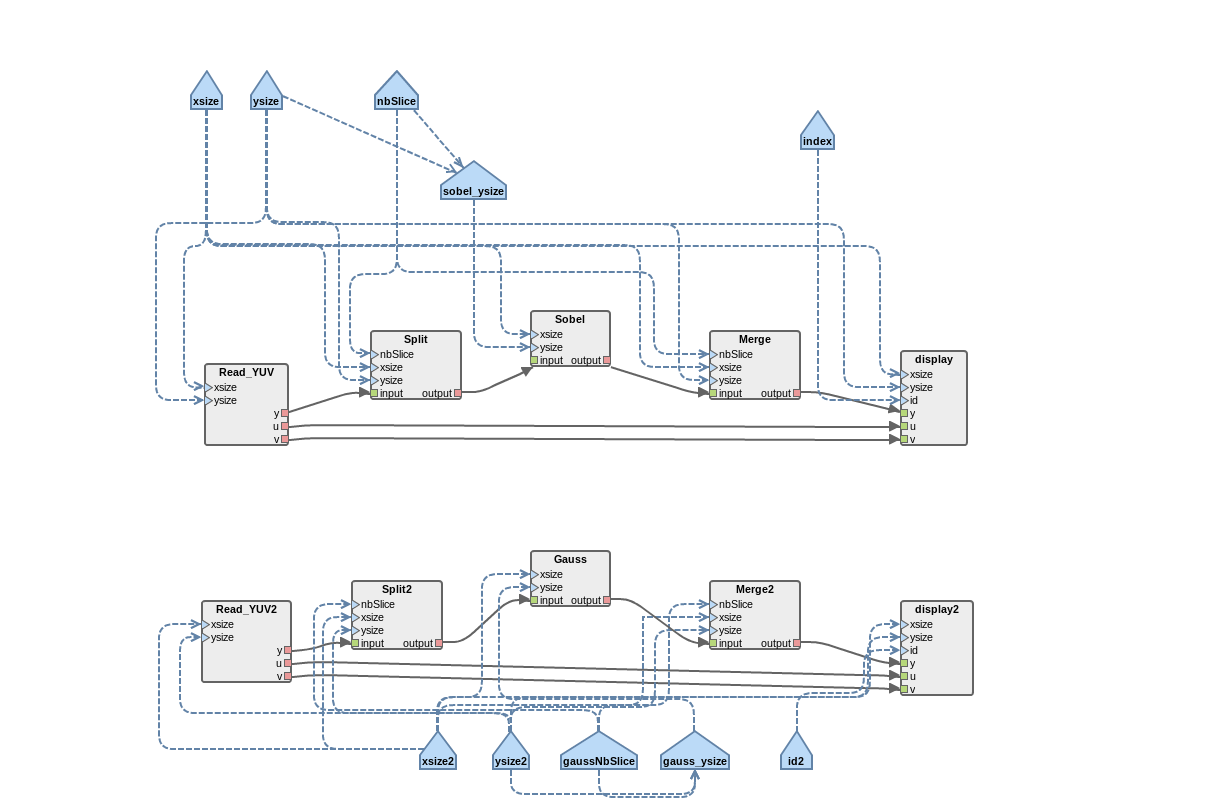
\includegraphics[width=0.99\textwidth]{images/preesm_diagram.png}
    \caption{The PiSDF graph of the PREESM filter application} \end{center}
\end{figure}

To keep the model simple and the program well analyzable both of the processing
paths in the network are independent.

The first actor on both of the processing paths loads the video frames from
memory and passes them to splitting actors. The splitting actor splits the
frames to a suitable number of splices to enable processing of the same video
stream on multiple cores. The filter actor follows the splitting actor. Partial
frames filtered in the filter actor are merged back to whole frames in the merge
actors. The last actors on both of the processing paths are dummy actors.\\

TODO: explain scheduling

\section{OpenEM Filter Application}
The OpenEM implementation of the filter application was heavily influenced by
the PREESM filter application described in \ref{sec:preesmapp}. Specifically the
OpenEM application has to process the frames in similar manner so that only the
scheduling policies between the two programming models should differ. The PREESM
application splits the frames into slices and processes the slices separately
before merging them back into one frame. Similar fork-join mechanism was
implemented in the OpenEM application. Event groups were first planned to be
used as the fork-join mechanism in the filter application but in the final
implementation a different, simpler mechanism was used.

The TI implementation of event groups lacks \texttt{em\_event\_group\_delete}
function which makes it necessary to reuse the existing event groups. The
example applications which are included in the NSN OpenEM distribution described
in \ref{openemframework} demonstrate reuse of event groups, but it was estimated
that the programming overhead resulting from the reuse of the groups would be
larger than implementing the fork-join in a simpler manner.

In the final implementation the frames are accumulated simply in a merge buffer
located in shared memory which is referenced through queue context pointers. The
book keeping for frame completion is handled in the same location. The cache
coherency for the book keeping was handled by marking the memory area the merge
buffer resides in as non-cacheable.

\section{PSE Model of OpenEM Filter Application}
\section{Instrumentation}
